% PALM Workshop revision of "The Song, Not the Pin".
% Main text is translated from the Russian author rewrite.
\documentclass{article}
\usepackage[dblblindworkshop]{neurips_2026}
\workshoptitle{PALM: Personalized, Aligned, Long-Term Memory for AI Systems}

\usepackage[utf8]{inputenc}
\usepackage[T1]{fontenc}
\usepackage{hyperref}
\hypersetup{hidelinks}
\usepackage{url}
\usepackage{booktabs}
\usepackage{amsfonts}
\usepackage{amssymb}
\usepackage{amsmath}
\usepackage{nicefrac}
\usepackage{microtype}
\usepackage{xcolor}
\usepackage{graphicx}
\usepackage{array}
\usepackage{enumitem}
\usepackage{placeins}
\usepackage{flafter}
\usepackage{tikz}
\usetikzlibrary{arrows.meta,positioning,fit}
\graphicspath{{figures/}}

\setlength{\textfloatsep}{8pt plus 2pt minus 2pt}
\setlength{\floatsep}{8pt plus 2pt minus 2pt}
\setlength{\intextsep}{8pt plus 2pt minus 2pt}
\setlength{\abovecaptionskip}{4pt}
\setlength{\belowcaptionskip}{-2pt}

\newcommand{\mstar}{M^{\star}}
\newcommand{\cstar}{C^{\star}}
\newcommand{\fstar}{F^{\star}}
\newcommand{\rfstar}{RF^{\star}}
\newcommand{\phiroute}{\varphi_{\mathrm{route}}}
\newcommand{\method}[1]{\texttt{#1}}
\newcolumntype{L}[1]{>{\raggedright\arraybackslash}p{#1}}

\title{The Song, Not the Pin: Provenance-Conditioned Route Memory for Persistent Multi-Agent Navigation}
\author{Anonymous Author(s)}

\begin{document}
\maketitle

\begin{abstract}
Long-term memory becomes genuinely useful not at the moment of storage, but at the moment when a stored record begins to determine a subsequent action. In a multi-agent system this transition is especially problematic: a record may be semantically correct while still referring to an ambiguous place, lacking an executable path, being stale, or driving several agents toward the same scarce target. In this work we study shared long-term memory exactly at this level, as a mechanism that must not only return content but also justify why acting on that content is currently admissible.

We introduce an action-level memory contract in which the transferable unit is an executable route with explicit data provenance; a single target record is treated as a degenerate route of length zero. For each commitment we freeze the foreign-evidence share at the moment the target is materialized. Source trust and record age define a computable validity horizon, and the same principle is extended to individual route edges. For conflicting commitments we use a decentralized reservation-and-rollback protocol that makes memory's right to affect action conditional and revocable.

Experiments in grid environments, a continuous VMAS setting, and a small text world show that foreign memory has no single sign of effect. Under target scarcity, foreign commitments rarely complete directly, but often transport the agent into a region where self-confirmation becomes possible. Paired deterministic replay that masks only foreign evidence shows that sharing accelerates goal achievement in some regimes and degrades it in others because of coordination conflict. The trust--staleness threshold exactly predicts registered target hold-out breakpoints and all 110 tested route-memory rupture regimes; 21 intermediate ruptures are localized to the exact edge. Route transfer preserves success where transfer of the endpoint alone fails at the first structural obstacle. In a cross-session LLM experiment, a new agent solves 10/10 tasks with foreign long-term memory and 0/10 without it.

The claim we support is intentionally narrow: shared long-term memory should not be represented only as retrievable content. To become action, a record must have referential identity, execution structure, explicit provenance, time-bounded validity, and revocable coordination authority.
\end{abstract}

\section{Introduction}

Long-term memory systems are increasingly expected to do more than store information beyond a single context window. Memory should survive across sessions, be retrieved correctly after long delays, be updated when new data arrive, and participate in later decisions. Modern systems have made substantial progress on storage, retrieval, consolidation, and forgetting for conversational and embodied agents \citep{packer2023memgpt,park2023generative,zhong2024memorybank,wang2023voyager,xu2025amem,chhikara2025mem0}. At the same time, LoCoMo and LongMemEval show that long-term memory is not reducible to increasing the amount of available context: temporal reasoning, cross-session use, update, and correct refusal remain separate failure modes \citep{wu2024longmemeval,maharana2024locomo}.

In a multi-agent system there is an additional layer. An agent may receive a correct record from another agent's memory and still lack a sufficient basis for acting on it. Successful retrieval answers the question ``what is known,'' but it does not answer the question ``can this knowledge now be turned into action.'' This distinction is central to our formulation.

Consider a record stating that another agent discovered a water source. For this record to become executable for a recipient, five properties must be checked (Table~\ref{tab:intro-contract}). A semantically correct memory can fail along any of the other axes.

\begin{table}[t]
\caption{Action-level requirements for turning a retrieved foreign record into behavior.}
\label{tab:intro-contract}
\centering
\small
\begin{tabular}{L{0.20\linewidth}L{0.36\linewidth}L{0.34\linewidth}}
\toprule
Property & Question & Failure if missing \\
\midrule
Identity & What local referent does this record denote? & phantom or wrong target \\
Transport & How does the agent get there? & destination-only failure \\
Provenance & Who supports this claim? & untrusted or unattributed lock \\
Validity & Is the evidence still admissible? & stale target or stale edge \\
Authority & May this agent act on it now? & duplicate commitment or collision \\
\bottomrule
\end{tabular}
\end{table}

We combine these properties into an action-level memory contract. The experimental setting remains deliberately controlled: each agent has private memory, exchange occurs through explicitly specified communication topologies, merge rules are available for analysis, target scarcity is set directly, and planner commitments are logged. Such an environment allows us to measure memory content, provenance, validity expiration, and action conflict separately, rather than mixing them into a single end-to-end success rate.

The main object of the work is an executable route with data provenance. A target record is its degenerate length-zero case. This matters because memory of the correct point does not guarantee that the agent can reach it, and a route, in turn, may remain valid only partially. We therefore extend provenance and temporal admissibility from place records to transition structure.

The paper makes four main contributions. First, we freeze provenance directly at the moment of target materialization and separate the descriptive foreign-evidence share from the system-level counterfactual effect of removing it via paired deterministic replay. Second, an explicit trust--staleness rule yields an admissibility horizon for a record, and the same contract is then applied to individual route edges. Third, we show that the negative effect of fast sharing under target scarcity arises not only from information quality but also from conflicting commitments, and we introduce a decentralized reservation-plus-rollback protocol. Fourth, we weaken the shared-coordinate-frame assumption through semantic alignment of local landmarks and demonstrate cross-session use of foreign memory in a small LLM world.

We do not claim a general theory of long-term memory, and we do not interpret controlled environments as a universal benchmark. Their role is to isolate properties that are hard to observe separately in full end-to-end LLM systems. The main conclusion is therefore architectural: transferable memory should not be an automatically trusted fact, but a provenance- and validity-bounded basis for action.

\begin{figure}[t]
\centering
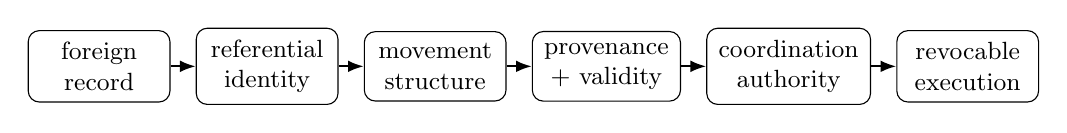
\begin{tikzpicture}[font=\small, node distance=4mm and 3.2mm,
box/.style={draw,rounded corners,align=center,minimum height=8mm,minimum width=18mm,inner sep=1.5mm},
arr/.style={-{Latex[length=2mm]},thick}]
\node[box] (record) {foreign\\record};
\node[box,right=of record] (id) {referential\\identity};
\node[box,right=of id] (route) {movement\\structure};
\node[box,right=of route] (valid) {provenance\\+ validity};
\node[box,right=of valid] (coord) {coordination\\authority};
\node[box,right=of coord] (act) {revocable\\execution};
\draw[arr] (record)--(id); \draw[arr] (id)--(route); \draw[arr] (route)--(valid); \draw[arr] (valid)--(coord); \draw[arr] (coord)--(act);
\end{tikzpicture}
\caption{The action-level memory contract. Semantic relevance is only the first condition. For foreign long-term memory to become executable, the recipient additionally needs an unambiguous referent, action structure, provenance and evidence lifetime, and a rule that determines whether the record may control action in the current system state.}
\label{fig:contract}
\end{figure}

\section{Long-term foreign memory as authority to act}

\paragraph{Memory substrate.}
Each agent maintains its own symbolic memory of visited places. A record contains semantic tags, confidence, amount of supporting evidence, freshness, source identifier, and transition statistics. We compare five memory organizations: independent private memories, a shared event bus, a central aggregator, peer-to-peer broadcast every $K$ ticks, and Collective Semantic Memory (CSM), where the merge explicitly accounts for trust and staleness. In all variants the planner and local controller are identical; only the memory topology and evidence-merge contract change.

The main grid environment is a partially observed $12\times 10$ space with $N$ agents and $T<N$ semantic targets of the ``water source'' type. Target scarcity is intentional: it lets us separate the usefulness of shared information from the coordination cost of multiple agents receiving the same basis for action.

\paragraph{Observable stages of memory use.}
At every tick we log four events: query formation, successful semantic retrieval, target materialization, and completion. These events are used as a measurement interface, not as a separate contribution of the paper. The central event for this article is $\mstar$: the planner has converted a retrieved candidate into a concrete locked target. Event $\cstar$ means that the locked target has been reached. Thus $\mstar$ defines the observable moment at which a record moves from ``available'' to ``authorized to guide action.''

\paragraph{Provenance at commitment time.}
Every evidence item $e$ retains a source $\pi(e)$. For candidate $m$ selected at $\mstar$, the foreign-evidence share is defined as
\begin{equation}
\varphi(m)=
\frac{\sum_{e\in \mathrm{supp}(m),\,\pi(e)\neq\mathrm{self}} w(e)}
{\sum_{e\in \mathrm{supp}(m)} w(e)} .
\label{eq:phi}
\end{equation}
Here $w(e)$ is the actual evidence weight in the merge mechanism, not a post-hoc attribution score. For CSM,
\[
w(e)=\tau_i \exp(-\alpha\,\mathrm{age}(e))\,c(e),
\]
where $\tau_i$ is trust in source $i$, $c(e)$ is evidence confidence, and $\alpha$ is the decay rate. The value of $\varphi$ is frozen when the target is locked. If the agent later confirms the target itself, that confirmation does not rewrite the provenance of the decision that initially moved the agent toward it.

A commitment based on foreign memory is defined as
\[
F^*_{\theta}=\mstar \wedge [\varphi\geq\theta].
\]
The main descriptive analysis uses $\theta=0.8$; the strict variant requires $\varphi=1$. Importantly, $\varphi$ is not a causal quantity. A large foreign-evidence share may be redundant if the agent had equivalent self evidence. A small external contribution may conversely change the selected target. Provenance mass and the counterfactual effect of removing foreign memory are therefore analyzed separately.

\paragraph{Temporal validity.}
The same merge contract gives an explicit admissibility horizon. Foreign evidence participates in retrieval while
\[
\tau_i c \exp(-\alpha\,\mathrm{age})>\tau ,
\]
where $\tau$ is the inclusion threshold. Hence the maximum admissible age is
\begin{equation}
\mathrm{age}_{\max}(\tau_i,c)=\frac{1}{\alpha}\log\frac{\tau_i c}{\tau},
\qquad \tau_i c>\tau .
\label{eq:horizon}
\end{equation}
This is not a learned law of the environment, but a direct consequence of the chosen contract. Its practical meaning is that a record has a computable condition after which it should no longer serve on its own as a basis for action.

\paragraph{Authority states.}
For foreign evidence we distinguish four states: the record has been observed by its source; the record has been received by another agent; the record is conditionally executable under identity, transport, validity, and coordination checks; and the record has been confirmed by the recipient itself. The present work mainly studies the third state. Foreign memory may temporarily guide behavior before self-confirmation, but this right is bounded and can be revoked.

\section{Experimental design}

The experiments are designed not to conflate the presence of a memory record with its actual influence on action. In each block, where possible, we change one layer of the contract while leaving the remaining components of the stack fixed.

The main target-provenance sweep includes 2,400 paired episodes: five $(N,T)$ regimes, three environment configurations, four memory architectures, 20 seeds, and two replay conditions. The first run uses full memory. In the second, only foreign evidence is masked at the merge stage under the same seed and initial random stream. This comparison estimates not the presence of foreign information as such, but the system-level change after removing it.

For the peer-to-peer architecture we separately vary the exchange frequency $K\in\{1,2,4,8,16\}$. The reservation-plus-rollback intervention is evaluated on 840 episodes at $K\in\{1,2,4\}$; $K=8$ is used as a fixed strong comparison point. Confidence intervals are computed with an episode-cluster bootstrap.

Validity is tested in a witness--traveler protocol. The witness observes a target once and then transmits no new data. The traveler receives a memory snapshot after a controlled delay. The content of the evidence is fixed; only its age changes. The last admissible moment predicted by Equation~\ref{eq:horizon} is compared with a registered hold-out after which the agent should stop forming an intention from the record.

The route block tests whether transmitting a destination is sufficient or whether movement structure is required. We use mazes of size $12\times 10$ to $14\times 12$ with obstacles and hazards. Three regimes are compared: destination-only, route transfer, and blind exploration. For validity of individual edges we use five mazes, 11 delays, and two trust levels, for 110 regimes total. In each regime we check whether the factual first inadmissible edge matches the computed rupture index.

A separate block removes the shared-coordinate-frame assumption. Unknown translations and quarter-turn rotations are imposed between agents, and place correspondence is recovered from the semantic structure of local landmarks. A continuous VMAS experiment checks whether the observed effect of exchange frequency persists outside the discrete grid; it is used as a portability check rather than as a separate leaderboard benchmark.

The language experiment is intentionally small. A local LLM extracts semantic tags from natural-language observations in a three-room text house, after which symbolic memory is saved to disk. In the second session, a new agent loads this memory solely as foreign provenance. The LLM selects the semantic target and take/put decisions, while low-level movement after materialization is executed by a deterministic controller. This design isolates cross-session memory use from locomotion errors.

\section{What foreign memory contributes}

\paragraph{Direct completion is rare under target scarcity.}
Table~\ref{tab:provenance} shows a large gap between commitments based mainly on foreign evidence and commitments based on self observation. Under fast peer-to-peer exchange, only 0.4\% of foreign locks directly complete by reaching the target, compared with 22.3\% of own locks. The same qualitative pattern persists across architectures.

This gap should not be read as evidence that foreign memory is semantically wrong. The two layers arise in different states. A foreign lock is formed at an average distance of 6.26 cells from the target, while an own lock is formed at 1.15 cells. Mean simultaneous-lock pressure is 1.76 versus 0.21. Foreign memory therefore often operates earlier and serves as long-range transport, whereas self evidence appears only once the agent is already in the local confirmation region.

\begin{table}[t]
\caption{Completion under frozen provenance in scarcity episodes. Intervals are episode-cluster bootstrap CIs. The comparison is descriptive: groups are not matched on target distance, co-lock pressure, or other covariates.}
\label{tab:provenance}
\centering
\small
\begin{tabular}{lcc}
\toprule
Architecture & $P(\cstar\mid F^*_{0.8})$ & $P(\cstar\mid \mstar,\mathrm{own})$ \\
\midrule
peer $K=2$ & 0.004 [0.001, 0.008] & 0.223 [0.186, 0.275] \\
peer $K=8$ & 0.020 [0.000, 0.038] & 0.389 [0.329, 0.446] \\
CSM $K=8$ & 0.017 [0.006, 0.044] & 0.414 [0.368, 0.453] \\
shared bus & 0.004 [0.002, 0.008] & 0.279 [0.237, 0.332] \\
\bottomrule
\end{tabular}
\end{table}

\paragraph{Foreign memory often acts as transport.}
We call an own completion foreign-supported if, in the same episode and for the same agent, it was preceded by a removed foreign lock on the same target. For the shared bus, this chain appears in 127 of 248 own completions (51.2\%); for peer $K=2$, in 99 of 223 (44.4\%). The first foreign lock occurs approximately 8--10 cells from the target, and the final own lock occurs around 2.0 cells, that is, inside the self-confirmation radius.

This statistic shows precedence, not causality. It explains only the mechanism: a foreign record may fail to complete the task directly, yet move the agent into the region where self evidence becomes available. The provenance of the decision must therefore be separated from the factual contribution of foreign memory.

Paired replay does exactly this. We mask foreign evidence at the merge stage and repeat the same seed. After the intervention, actions may diverge, so the estimand is a system-level counterfactual effect rather than a mediation effect for an individual $\mstar$.

The sign of the effect depends on the regime. Under moderate scarcity and the shared bus, foreign memory improves censored time to success by $+10.8$ ticks [+$2.2$, +$20.9$]. Under fast peer-to-peer exchange the effect becomes negative: for $K=2$ it is $-7.1$ ticks [$-13.5$, $-1.3$]. If foreign memory is masked for only one recipient, the sign remains the same: $-10.25$ ticks [$-20.91$, $-0.16$], while spillover to the other agents remains approximately zero.

Thus the correct conclusion is not that foreign memory ``helps'' or ``hurts'' in itself. Its informational value and coordination cost are different quantities. The same accurate record can be useful as a source of long-range direction and simultaneously degrade the system if several agents receive the same basis for competitive action.

\section{Validity and coordination of long-term memory}

\paragraph{The staleness threshold predicts when authority expires.}
Equation~\ref{eq:horizon} is tested without additional fitting. In the witness--traveler setting, the measured last age at which the target still participates in retrieval coincides with the analytical threshold crossing for every tested trust level.

In full navigation episodes, the registered hold-out also correctly predicts all 6/6 completion-change points. The set includes ordinary breakpoints, a regime in which the record is never admissible, and a regime where storage pruning occurs before the exponential threshold. Thus $\mathrm{age}_{\max}$ is interpreted as an invariant of the concrete contract implementation, not as an empirical law transferable to arbitrary memory models.

\begin{figure}[t]
\centering
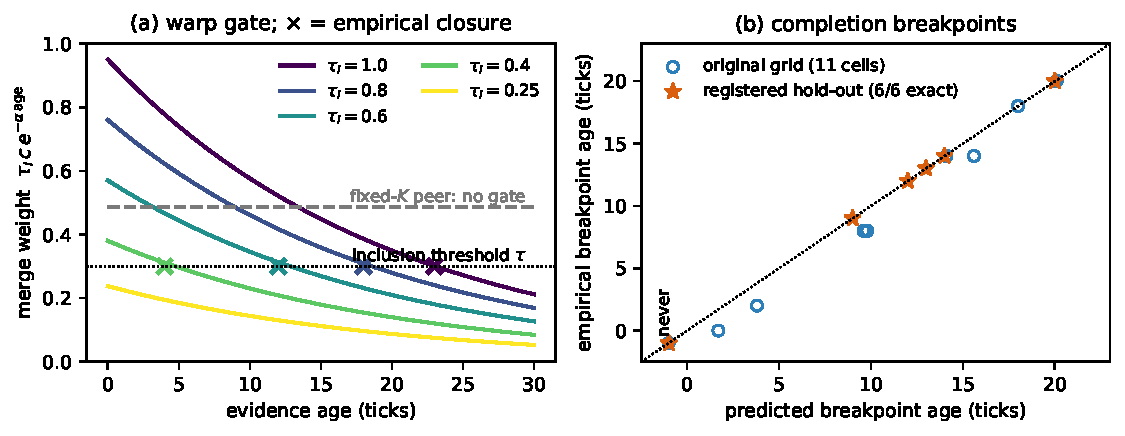
\includegraphics[width=.94\linewidth]{fig_warp_law.pdf}
\caption{Validity horizon for long-term foreign evidence: analytical trust--staleness threshold and registered hold-out breakpoints.}
\label{fig:warp-law}
\end{figure}

\paragraph{Fast sharing creates a separate coordination failure.}
The counterfactual analysis shows that the negative effect at small $K$ is concentrated in duplicated commitments to the same scarce target. The record content can be correct and fresh. The error arises later: several agents simultaneously obtain a sufficient basis for the same action.

For this regime we add a decentralized reservation-plus-rollback protocol without changing semantic content or retrieval. An agent may optimistically lock a target; the next ordinary peer message carries a reservation; if a local lock is dominated by an existing reservation, it is removed and the query is repeated after exponential backoff. Priority is determined deterministically by lock time, distance to the target at lock time, and agent identifier. No central coordinator or additional communication channel is introduced. In spirit, the mechanism is close to optimistic rollback in Time Warp \citep{jefferson1985}.

\begin{table}[t]
\caption{Reservation-and-rollback intervention. The protocol improves success at every tested high exchange frequency and in all three cases exceeds the fixed $K=8$ baseline in unconditional success.}
\label{tab:coord}
\centering
\small
\begin{tabular}{lcc}
\toprule
Regime & Success & Censored $t_{\mathrm{succ}}$ \\
\midrule
$K=1$: baseline / protocol & 0.592 / \textbf{0.620} & 55.3 / \textbf{53.1} \\
$K=2$: baseline / protocol & 0.572 / \textbf{0.614} & 57.2 / \textbf{53.2} \\
$K=4$: baseline / protocol & 0.577 / \textbf{0.620} & 57.3 / \textbf{52.2} \\
$K=8$: fixed baseline & 0.583 & 55.2 \\
\bottomrule
\end{tabular}
\end{table}

This result changes the interpretation of the ``optimal'' $K$. Without an explicit coordination interface, moderate exchange frequency partly works as an implicit rate limiter: information spreads quickly enough to be useful, but slowly enough to limit the number of simultaneous conflicting locks. After revocable authority is introduced, fast exchange no longer has to pay the same price at the completion stage.

For multi-agent memory, the important point is to distinguish two operations. The first determines what an agent knows and can retrieve. The second determines whether, in the current system state, the agent is allowed to turn that knowledge into a commitment. Our protocol tests exactly the second interface. At the same time, reservation, rollback, and backoff are evaluated as one linked mechanism; the work does not identify the contribution of each primitive separately. A broader 2,520-episode coordination-baseline sweep compares this linked mechanism against five decentralized alternatives using the same broadcast information (Appendix~\ref{app:coord-baselines}); this supports a bounded advantage of the full authority interface, not dominance of any single primitive.

\begin{figure}[t]
\centering
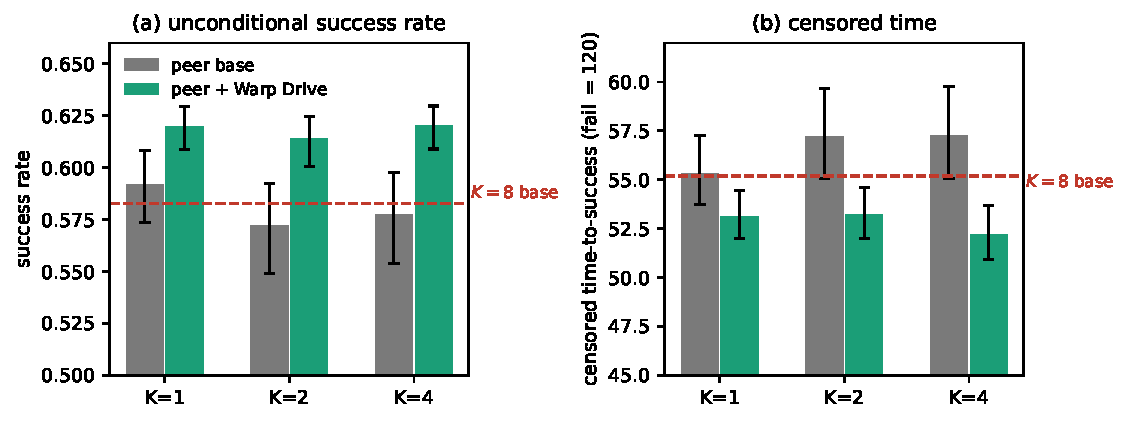
\includegraphics[width=.88\linewidth]{fig_warp_drive.pdf}
\caption{Reservation-plus-rollback intervention: fast exchange is preserved, but memory's right to control action becomes revocable.}
\label{fig:warp-drive}
\end{figure}

\FloatBarrier
\section{From target records to executable route memory}

A target record can be semantically correct and operationally incomplete at the same time. Knowing ``where the goal is'' is not equivalent to knowing ``how to get there.'' We therefore extend provenance and validity from individual places to route edges.

The transmitted snapshot contains only edges that the sender actually traversed itself. Foreign edges are not rebroadcast. This contract preserves the original source of every transition and prevents cascading reuse of routes whose provenance has been lost.

For a committed path $P$, the foreign route-evidence share is
\begin{equation}
\phiroute(P)=
\frac{\sum_{e\in P,\,\pi(e)\neq\mathrm{self}} w(e)}
{\sum_{e\in P} w(e)},\quad
w(e)=\tau_i \exp(-\alpha\,\mathrm{age}(e))\log(1+\mathrm{count}(e)).
\label{eq:routephi}
\end{equation}
Here $\tau_i$ is source trust, $\mathrm{age}(e)$ is the age of the transition evidence, and $\mathrm{count}(e)$ is the number of confirmed traversals. A strict foreign route is a connected previously traversed subpath of at least five edges with $\phiroute=1$.

\paragraph{A destination without movement structure can be worse than no memory.}
In a comb maze with detour factor $D=2.65$, the traveler follows a fully foreign 45-edge route and completes the task in 54 ticks. With the same foreign target record but no edges, the standard local planner does not arrive within the 300-tick limit. Blind exploration in the same world takes 126 ticks.

On paired mazes, destination-only succeeds 20/20 in the unobstructed environment at $D=1.00$ and collapses to 0/20 already at the first structural obstacle, $D=1.38$. Route transfer remains 20/20 in every tested regime. The reason is not that the target is wrong: the coordinate remains correct, but it does not encode the topology of the detour. In our environments, Manhattan attraction toward the known point can even become actively harmful because it repeatedly pins the local planner against the blocking wall.

\begin{figure}[t]
\centering

\includegraphics[width=.94\linewidth]{fig_route_cliff.pdf}
\caption{A semantically correct endpoint is not always executable memory: route transfer preserves success after structural obstacles appear, while destination-only fails at the first such obstacle.}
\label{fig:route-cliff}
\end{figure}

\paragraph{A route has its own validity boundary.}
Because the witness traverses different edges at different moments, by execution time they have different ages. Reapplying the same trust--staleness gate while accounting for delay and traveler kinematics yields a rupture index: the first edge that should no longer be used as a basis for action.

Across five mazes, 11 delays, and two trust levels, the predictor matches all 110 qualitative regimes: full completion, intermediate rupture, or unusable from the first edge. All 21 intermediate ruptures occur exactly at the predicted edge; the index error is 0. This is the route analogue of Equation~\ref{eq:horizon}: relational memory may lose validity not globally, but locally along its own structure.

\paragraph{The valid prefix also preserves the witness's measured risk profile.}
In open environments with high hazard density, both route transfer and destination-only complete 20/20 tasks. But the agent following the route receives zero hazard hits in all 20 worlds, whereas destination-only produces a mean of 3.25 [2.45, 4.10] hits. In the rupture regime, no additional hits occur before the predicted edge; risk appears only after switching to the fallback policy.

We do not interpret this as a universal safety guarantee. The supported claim is narrower: the transferred route preserves the witness's measured risk profile on the part of the path that remains valid under the specified contract. The trust--staleness threshold itself does not guarantee safety beyond that prefix.

\FloatBarrier
\section{Private coordinate frames and cross-session language agents}

\paragraph{Meaning-based correspondence.}
A foreign coordinate is useless if agents do not share a reference frame. We therefore represent a place as a local semantic constellation: content landmarks such as water, hazards, and walls, together with their relative offsets around the visited cell. In this setting, identity is defined not by matching absolute coordinates but by the structure of local context.

A correspondence is accepted only when there is sufficient support. Candidate pairs must be mutually unique, contain at least two meaningful semantic keys, and support at least three agreeing landmark pairs. Translation is estimated from the modal offset. A quarter-turn rotation is selected only when its consensus unambiguously exceeds the nearest alternative. Patterns consisting only of the world boundary are excluded: they encode environment shape rather than place identity.

Across 80 combinations of translation, rotation, offset, and seed, the semantic aligner recovers the discrete coordinate frame exactly in 80/80 cases and completes every strict foreign-memory transfer. In deliberately constructed ambiguous worlds, by contrast, it refuses to materialize a target. The raw-coordinate baseline continues to lock a concrete but wrong cell. We treat this as the correct fail-closed behavior: lack of sufficient support should lead to refusal, not forced materialization.

In an online setting with $N=4$ and target scarcity, the shared-frame oracle reaches success 0.456. Raw coordinates after misalignment yield 0.350. Semantic correspondence restores success to 0.444, closing about 88\% of the gap. After referent recovery, the temporal-validity boundary is unchanged. Within these experiments, identity and staleness behave as separable contract layers: the first answers which place the record refers to, and the second answers whether the corresponding record may still be acted upon.

\paragraph{Cross-session LLM memory.}
In session 1, agent A receives natural-language observations, and a local LLM converts them into semantic tags. Symbolic memory is saved to disk. In session 2, a new agent B loads this dump as entirely foreign memory and performs the task ``bring the apple to the table'' without the standard directional oracle.

With foreign long-term memory, B completes 10/10 randomized configurations with mean time 8.3 ticks. With empty memory, it completes 0/10. Every long-range lock on the apple or table before local confirmation has $\varphi=1$. This experiment shows that a record can cross not only an agent boundary but also a session boundary while retaining measurable provenance.

A small live collective of $N=3$ language agents reproduces the same coordination failure. With two scarce apples, direct exchange reduces the number of successful agents on paired configurations from $2/3$ to $1/3$. Adding reservation plus rollback increases pooled success from 0.333 to 0.417 at both tested exchange frequencies. Recovery remains partial: hallucinated semantic anchors and noisy locks lie outside the coordination module.

This residual negative result is useful because it separates two different failure classes. The first concerns content: an LLM may store or retrieve an incorrect semantic anchor. The second concerns authority: several agents may receive a correct record and still use it in a conflicting way. A scalar success rate mixes these mechanisms; an explicit contract makes them distinguishable.

\begin{table}[t]
\caption{Controlled checks of the action-level memory contract.}
\label{tab:contracttests}
\centering
\small
\begin{tabular}{L{0.19\linewidth}L{0.30\linewidth}L{0.39\linewidth}}
\toprule
Requirement & Stress test & Main observation \\
\midrule
Transport & destination-only vs. route memory & At the first structural obstacle ($D=1.38$): route 20/20; destination-only 0/20. \\
Validity & delayed edge evidence & 110/110 correct regimes; all 21 intermediate ruptures localized exactly. \\
Identity & private translations and rotations & 80/80 exact recoveries; ambiguous worlds rejected instead of erroneous materialization. \\
Persistence & cross-session LLM memory & foreign memory 10/10; empty memory 0/10. \\
Coordination & fast exchange under target scarcity & reservation plus rollback improves success at every $K\in\{1,2,4\}$. \\
\bottomrule
\end{tabular}
\end{table}

\begin{table}[t]
\caption{Positioning relative to contemporary memory and agent-system paradigms. ``Validity'' means temporal admissibility; ``CF'' denotes paired counterfactual estimation. The table does not claim superiority as a mapper, communication policy, or universal memory store; it shows which fields are made explicit specifically at the transition from a foreign record to action.}
\label{tab:positioning}
\centering
\scriptsize
\setlength{\tabcolsep}{2.4pt}
\begin{tabular}{lcccccc}
\toprule
Paradigm & identity & route & prov. & validity & coord. & CF \\
\midrule
LLM memory stores/evals & -- & -- & $\pm$ & $\pm$ & -- & -- \\
Embodied skill/episodic memory & -- & $\pm$ & -- & -- & -- & -- \\
Shared maps/place recognition & \checkmark & \checkmark & -- & $\pm$ & $\pm$ & -- \\
Learned multi-agent communication & -- & -- & -- & -- & \checkmark & -- \\
This work & \checkmark & \checkmark & \checkmark & \checkmark & \checkmark & \checkmark \\
\bottomrule
\end{tabular}
\end{table}

\section{Related work}

\paragraph{Long-term memory for language agents.}
Modern memory systems for language agents mainly address storing and reusing information beyond a single context window. MemGPT organizes multiple memory levels and manages information transfer between them \citep{packer2023memgpt}. MemoryBank introduces explicit update and forgetting mechanisms \citep{zhong2024memorybank}. Generative Agents combine a long-term experience stream with retrieval and reflection \citep{park2023generative}. A-MEM represents memory as an evolving linked structure \citep{xu2025amem}, and Mem0 studies scalable extraction, consolidation, and graph-enhanced long-term memory \citep{chhikara2025mem0}.

These works primarily answer the questions of what to store, how to organize it, when to retrieve it, and how to update it. Our formulation is at the next step: what must accompany an already retrieved record, if it was created by another agent, before that record can determine action, and under what conditions should this right be revoked?

\paragraph{Evaluation of long-term memory.}
LoCoMo and LongMemEval show that long-term-memory quality cannot be reduced to factual reproduction of a short context. Temporal reasoning, cross-session transfer, knowledge update, and correct refusal must be tested separately \citep{maharana2024locomo,wu2024longmemeval}.

We add an action-level axis. Retrieval may be semantically correct and still non-executable: the referent may be ambiguous, the route may be missing, the evidence may become stale, or the action may conflict with another commitment. This is close in spirit to abstention, but the basis for refusal here is not only answer uncertainty; it is an explicit identity, provenance, transport, validity, and coordination contract.

\paragraph{Embodied and multi-agent memory.}
In embodied systems, memory is also used for later behavior. Voyager stores reusable executable skills \citep{wang2023voyager}, and Reflexion carries episodic linguistic feedback across attempts \citep{shinn2023reflexion}. In multi-agent learning, CommNet and TarMAC learn communication representations for coordination \citep{sukhbaatar2016commnet,das2019tarmac}.

Our object differs in that transmitted long-term records remain inspectable after communication. For a decision, one can recover the source, age, evidence weight, and, for route memory, the concrete transitions. This makes it possible to analyze not just communication, but the moment when a message becomes a commitment.

The work is also related to SLAM and visual place recognition, where mature methods solve geometric map merging, loop closure, and place matching \citep{cadena2016slam,lowry2016vpr}. Our discrete semantic alignment is substantially narrower and is not proposed as an alternative to full mapping. It is used only to isolate one question: whether the referential identity of foreign memory survives without a shared absolute coordinate frame.

\section{Limitations and discussion}

The strongest part of the evidence base is the controlled mechanism study. Most experiments use grid environments with a predefined semantic vocabulary. VMAS and the text world serve as portability checks for individual effects, not as broad performance benchmarks.

The LLM experiment is small in scale and uses deterministic locomotion after semantic-target selection. We do not study open-ended memory editing by the language model, adversarial memory poisoning, deletion at user request, or long-term memory evolution across many sessions. These scenarios may create additional error channels absent from the current implementation.

Private coordinate frames are limited to translations and quarter-turn rotations; arbitrary continuous $SE(2)$ transformations are not considered. Semantic landmarks are specified manually at the environment level rather than extracted from raw observations by a learned visual model. Thus the experiments test the identity contract, but they do not solve general visual place recognition.

The coordination intervention is also evaluated as a single protocol. We do not have separate ablations for reservation-only, rollback-only, backoff-only, or a centralized oracle. The observed gain therefore supports the usefulness of a revocable authority interface as a whole, but it does not attribute the effect to an individual component.

The horizon formula and edge-rupture predictor are exact because they are consequences of the concrete exponential trust--staleness gate and pruning schedule. This is a test of internal consistency for the implemented contract, not evidence that exponential decay is a universally correct memory model. For a learned or nonlinear forgetting rule, the boundary may have a different form.

It is also important to distinguish the causal status of the results. The completion gap between own and foreign commitments is descriptive and does not control covariate imbalance. Chains of ``foreign lock $\to$ self confirmation $\to$ completion'' show precedence but not causality. Masked replay is a paired system-level intervention, but after divergence the agents' trajectories affect each other. Reservation plus rollback is a module-level intervention. Validity boundaries are predictions of the contract itself, checked against the implementation.

We preserve these distinctions deliberately. The phrase ``memory helped'' is too coarse if it simultaneously mixes provenance, causal contribution, and memory's right to control action. For a long-term memory architecture it is more useful to distinguish two interfaces. The content interface answers what the system stored and can retrieve. The authority interface answers why a particular record may currently affect action and when that right should be revoked.

In a multi-agent system, the authority interface naturally includes source, expiration, referential correspondence, execution structure, and coordination state. Our stress tests show that these fields are not cosmetic metadata: violating each one creates a distinct observable failure mode.

Finally, under ambiguous correspondence we use a fail-closed decision: the target is not materialized if support is insufficient. The work does not construct the full coverage--fail-open trade-off and does not determine the optimal boundary between refusal and the risk of erroneous materialization. This result should be read as a demonstration of a separate failure mode, not as a complete theory of abstention for memory.

\section{Conclusion}

We studied shared long-term memory at the point where retrieved information becomes action. At that point, one semantically correct record is not enough. For foreign memory to become executable, the agent must understand what the record refers to, know an admissible movement structure, account for the evidence source, check its temporal validity, and be able to revoke the commitment under coordination conflict.

The experiments show that foreign memory can be useful even when its probability of direct completion is almost zero. Its role is often long-range transport: it moves the agent into a region where self-confirmation appears. At the same time, the system-level sign of the effect is regime-dependent. Faster exchange increases information availability, but under target scarcity it also increases the probability of conflicting commitments.

The trust--staleness contract provides a computable moment after which foreign evidence should no longer be used. In route memory this principle becomes local: different edges may lose validity at different times. Reservation plus rollback shows that part of the loss under fast exchange is not about memory quality as such, but about the absence of an explicit mechanism for resolving conflicting rights to act.

Private coordinate frames and cross-session LLM memory show that the same language remains meaningful beyond the base grid. A record may survive boundaries between agents, world representations, and sessions, but that does not make it automatically trusted. The possibility of acting on it must still be checked separately.

The central design claim of the article is therefore intentionally limited: shared long-term memory should represent not only retrievable content, but also the conditions of its use. A transferable record should have explicit provenance, referential identity, time-bounded validity, and the necessary execution structure, and its right to affect action should remain conditional and revocable.

\FloatBarrier
\begin{thebibliography}{99}

\bibitem[Packer et~al.(2023)]{packer2023memgpt}
C.~Packer, S.~Wooders, K.~Lin, V.~Fang, S.~G. Patil, I.~Stoica, and J.~E. Gonzalez.
\newblock MemGPT: Towards LLMs as operating systems.
\newblock \emph{arXiv:2310.08560}, 2023.

\bibitem[Park et~al.(2023)]{park2023generative}
J.~S. Park, J.~C. O'Brien, C.~J. Cai, M.~R. Morris, P.~Liang, and M.~S. Bernstein.
\newblock Generative agents: Interactive simulacra of human behavior.
\newblock In \emph{UIST}, 2023.

\bibitem[Zhong et~al.(2024)]{zhong2024memorybank}
W.~Zhong, L.~Guo, Q.~Gao, H.~Ye, and Y.~Wang.
\newblock MemoryBank: Enhancing large language models with long-term memory.
\newblock In \emph{AAAI}, 2024.

\bibitem[Wu et~al.(2024)]{wu2024longmemeval}
D.~Wu, H.~Wang, W.~Yu, Y.~Zhang, K.-W. Chang, and D.~Yu.
\newblock LongMemEval: Benchmarking chat assistants on long-term interactive memory.
\newblock \emph{arXiv:2410.10813}, 2024. Accepted at ICLR 2025.

\bibitem[Maharana et~al.(2024)]{maharana2024locomo}
A.~Maharana, D.-H. Lee, S.~Tulyakov, M.~Bansal, F.~Barbieri, and Y.~Fang.
\newblock Evaluating very long-term conversational memory of LLM agents.
\newblock \emph{arXiv:2402.17753}, 2024.

\bibitem[Xu et~al.(2025)]{xu2025amem}
W.~Xu, Z.~Liang, K.~Mei, H.~Gao, J.~Tan, and Y.~Zhang.
\newblock A-MEM: Agentic memory for LLM agents.
\newblock In \emph{NeurIPS}, 2025.

\bibitem[Chhikara et~al.(2025)]{chhikara2025mem0}
P.~Chhikara, D.~Khant, S.~Aryan, T.~Singh, and D.~Yadav.
\newblock Mem0: Building production-ready AI agents with scalable long-term memory.
\newblock \emph{arXiv:2504.19413}, 2025.

\bibitem[Wang et~al.(2023)]{wang2023voyager}
G.~Wang, Y.~Xie, Y.~Jiang, A.~Mandlekar, C.~Xiao, Y.~Zhu, L.~Fan, and A.~Anandkumar.
\newblock Voyager: An open-ended embodied agent with large language models.
\newblock \emph{arXiv:2305.16291}, 2023.

\bibitem[Shinn et~al.(2023)]{shinn2023reflexion}
N.~Shinn, F.~Cassano, E.~Berman, A.~Gopinath, K.~Narasimhan, and S.~Yao.
\newblock Reflexion: Language agents with verbal reinforcement learning.
\newblock In \emph{NeurIPS}, 2023.

\bibitem[Sukhbaatar et~al.(2016)]{sukhbaatar2016commnet}
S.~Sukhbaatar, A.~Szlam, and R.~Fergus.
\newblock Learning multiagent communication with backpropagation.
\newblock In \emph{NeurIPS}, 2016.

\bibitem[Das et~al.(2019)]{das2019tarmac}
A.~Das, T.~Gervet, J.~Romoff, D.~Batra, D.~Parikh, M.~Rabbat, and J.~Pineau.
\newblock TarMAC: Targeted multi-agent communication.
\newblock In \emph{ICML}, 2019.

\bibitem[Cadena et~al.(2016)]{cadena2016slam}
C.~Cadena, L.~Carlone, H.~Carrillo, Y.~Latif, D.~Scaramuzza, J.~Neira, I.~Reid, and J.~J. Leonard.
\newblock Past, present, and future of simultaneous localization and mapping: Toward the robust-perception age.
\newblock \emph{IEEE Transactions on Robotics}, 32(6):1309--1332, 2016.

\bibitem[Lowry et~al.(2016)]{lowry2016vpr}
S.~Lowry, N.~S\"underhauf, P.~Newman, J.~J. Leonard, D.~Cox, P.~Corke, and M.~J. Milford.
\newblock Visual place recognition: A survey.
\newblock \emph{IEEE Transactions on Robotics}, 32(1):1--19, 2016.

\bibitem[Jefferson(1985)]{jefferson1985}
D.~R. Jefferson.
\newblock Virtual time.
\newblock \emph{ACM Transactions on Programming Languages and Systems}, 7(3):404--425, 1985.

\end{thebibliography}

\appendix

\section{Additional Materials and Experimental Details}

\subsection{Additional figures from the source manuscript}

\begin{figure}[h]
\centering
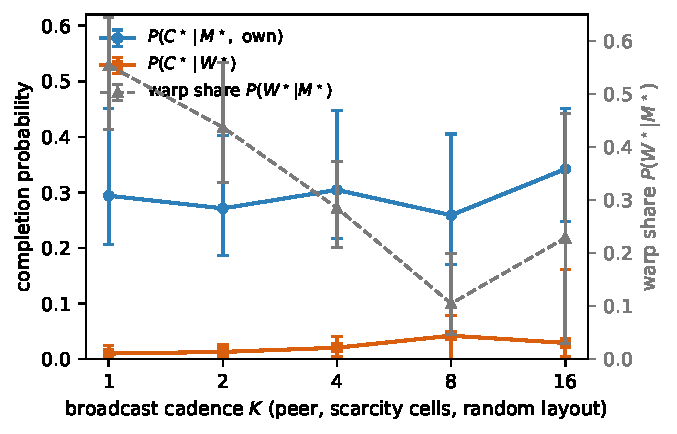
\includegraphics[width=.75\linewidth]{fig_warp_strata.pdf}
\caption{Completion probability stratified by commitment provenance, and the share of foreign locks as a function of peer-to-peer exchange frequency in target-scarcity scenarios.}
\label{fig:warp-strata}
\end{figure}

\begin{figure}[h]
\centering
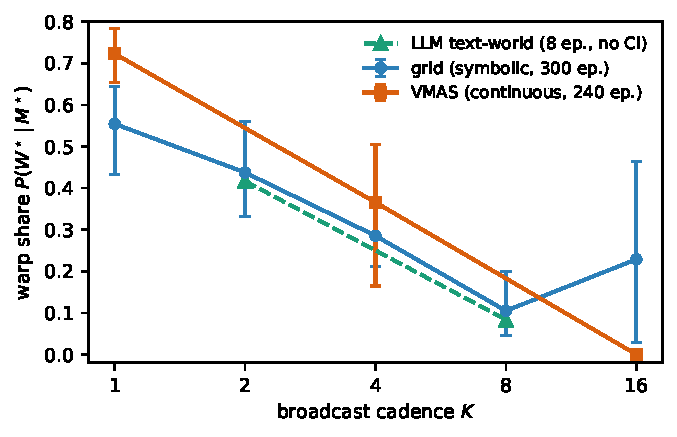
\includegraphics[width=.76\linewidth]{fig_warp_universality.pdf}
\caption{Foreign-commitment share as a function of exchange frequency on three substrates: symbolic grid, continuous VMAS, and LLM text world. This figure is used as a portability check for the observed trend, not as a unified cross-domain benchmark.}
\label{fig:warp-universality}
\end{figure}

\subsection{Threshold sensitivity and provenance bookkeeping}

The soft threshold $\theta=0.8$ is used only for stratification; the strict event requires $\varphi=1$. The pooled lock-level logs contain 23,237 events. The provenance-mass distribution is almost bimodal: most locks lie either near $\varphi=0$ or above 0.6. The most visible drop in completion occurs between the intervals $[0.4,0.6)$ and $[0.6,0.8)$, so the qualitative result does not depend on fine threshold tuning.

Because $\varphi$ is frozen at commitment time, a foreign lock can transport the agent into the observation region and then be removed and replaced by a self lock. The final completion is then correctly assigned to the later self commitment, while the preceding transport is accounted for separately through chain statistics.

Covariate imbalance between provenance layers is substantial: self locks are formed at an average distance of 1.15 cells from the target, foreign locks at 6.26; co-lock pressure is 0.21 versus 1.76. Matched analysis is possible only in a limited overlap region where foreign locks arise within two cells. There, the completion gap between self and foreign locks shrinks from 0.513 unadjusted to 0.38--0.45 within distance $\times$ co-lock strata. Therefore Table~\ref{tab:provenance} remains descriptive, and causal contribution is estimated only by intervention.

\subsection{Counterfactual estimands under interference}

Two replay quantities are used. The joint system effect removes foreign evidence from all agents while preserving the same random stream until divergence. The individual conditional effect removes foreign evidence only from agent $i$, while the other agents continue ordinary exchange. Because of multi-agent interference, neither quantity is a unit-level treatment effect in the SUTVA sense. They answer two narrower system questions: what contribution exchange makes to the collective, and what contribution foreign evidence makes to a particular recipient in the presence of spillover.

\subsection{Validity hold-out}

The witness--traveler protocol is first used on an exploratory parameter grid, after which a registered hold-out of six cells is formed. Predictions are written before execution. The hold-out includes ordinary endpoints, a cell that should never be admissible, and a pruning-limited cell where the storage horizon ends before Equation~\ref{eq:horizon}. All six outcomes match the implementation. This validates the contract and measurement procedure, but does not assert that exponential decay is the uniquely correct memory model.

\subsection{Additional coordination analysis}

The reservation is transmitted inside the ordinary peer snapshot at frequency $K$; no separate communication channel is introduced. If a local lock is dominated by a foreign reservation, it is removed, the target is temporarily suppressed by exponential backoff $4\to 8\to\cdots\to 32$ ticks, and the planner forms a query again. Direct per-agent calls without runtime reproduce the same rollback decisions from the local inbox, serving as a decentralization check.

Mean rollback latency approximately follows the exchange frequency: 1.0, 1.5, and 2.7 ticks for $K=1,2,4$, respectively. The protocol is evaluated by unconditional success and censored time because conditional completion denominators change when losing locks are removed before materialization. Normalized conditional ``recovery'' can exceed one relative to the scarcity ceiling, so the main claim is made only on unconditional task metrics.

\paragraph{Coordination-baseline sweep.}
\label{app:coord-baselines}
A separate 2,520-episode sweep compares the linked reservation-plus-rollback mechanism against five decentralized alternatives using the same broadcast information and identical seeds: random per-target priority, nearest-agent-wins, decentralized greedy assignment, exponential backoff without reservations, and a soft occupancy penalty. Table~\ref{tab:coord-baselines} summarizes the high-level outcome. Warp Drive is best or statistically tied on success at every tested cadence, but a single alternative can match or exceed it at an individual cadence. Its more consistent advantage is that it simultaneously preserves high success and gives the lowest duplicate-commitment count at every cadence. We therefore report this as a bounded systems advantage of the full authority interface, not as proof that any one primitive is uniquely necessary.

\begin{table}[h]
\caption{Decentralized coordination alternatives. Each cell reports success / duplicate-lock events per episode. ``Best alt.'' is the highest-success non-WD arm; ``lowest-dup alt.'' is the non-WD arm with the fewest duplicate-lock events.}
\label{tab:coord-baselines}
\centering
\scriptsize
\begin{tabular}{c L{0.16\linewidth} L{0.16\linewidth} L{0.24\linewidth} L{0.24\linewidth}}
\toprule
$K$ & none & Warp Drive & best alt. & lowest-dup alt. \\
\midrule
1 & 0.587 / 19.3 & 0.620 / 5.2 & backoff: 0.627 / 11.4 & backoff: 0.627 / 11.4 \\
2 & 0.570 / 18.8 & 0.611 / 4.5 & greedy: 0.612 / 15.9 & random: 0.608 / 5.9 \\
4 & 0.576 / 14.7 & 0.619 / 2.8 & greedy: 0.615 / 6.8 & random: 0.607 / 3.2 \\
\bottomrule
\end{tabular}
\end{table}

\subsection{Additional route-transfer results}

\paragraph{Breakdown of the destination-only regime.}
Three regimes are compared pairwise on identical mazes: route transfer, destination-only, and blind exploration. For detour factor $D\in\{1.00,1.38,2.03,3.32\}$, the route succeeds 20/20 in every interval. Destination-only succeeds 20/20 only at $D=1.00$ and 0/20 in all obstructed regimes. Blind exploration yields 20/20, 16/20, 17/20, and 15/20, respectively.

The gain of route transfer over destination-only in censored time is +4.7, +281, +273, and +262 ticks. The small difference at $D=1$ is explained by saving turns; the path length is the same in all 20 open cases.

\paragraph{Risk transfer.}
At hazard density 0.20 and with decay disabled to isolate the safety axis, both route transfer and destination-only complete 20/20 worlds. The foreign route has zero hazard hits in every world and mean time 16.6. Destination-only receives 3.25 [2.45, 4.10] hits with mean time 15.9. Blind exploration produces 28.7 hits on average.

In a separate composition with rupture, all 19 observed ruptures occur at the predicted edge. There are no hits before rupture; after switching to fallback, the mean number of hits is 0.58 [0.11, 1.32].

\begin{figure}[h]
\centering

\includegraphics[width=.82\linewidth]{fig_route_hazard.pdf}
\caption{Preservation of the risk profile on the valid prefix of a transferred route and resumption of risk after the predicted rupture.}
\label{fig:route-hazard}
\end{figure}

\subsection{Additional analysis of private coordinate frames}

A place fingerprint is defined as a local semantic constellation around the visited cell. A match is accepted only under mutual uniqueness above an exact-equality threshold. One-sided uniqueness is insufficient: the sender may know more places than the recipient, and a distant similar region may be incorrectly matched to a local neighborhood. Therefore at least two meaningful content keys and three agreeing pairs are required.

For rotations, each quarter-turn hypothesis is scored separately, and the winner must have at least twice the consensus of the nearest alternative. In translation-only worlds---four offsets, two hazard densities, and ten seeds---the hidden offset is recovered exactly in every run, with a mean of 15.1 mutual pairs.

For any nonzero offset, the raw-coordinate baseline locks a cell without water in every run; rare task success of 6.7\% arises from accidental route intersection. In featureless ambiguous worlds, the semantic mechanism creates no locks at all, while the coordinate baseline continues to materialize wrong targets. After adding rotations, exact recovery is 80/80. In a world with 180-degree symmetry, where the frame is in principle unidentifiable, the semantic matcher refuses all 10 locks, while the coordinate baseline creates 10/10 wrong ones.

A vocabulary ablation on 252 cells tests dependence on a rich hand-crafted alphabet. The full vocabulary, vocabulary without void, hazards-only, and vocabulary without walls all preserve 100\% exact recovery; removing hazards gives 92\%, walls-only gives 83\%, and void-only gives 0\%. No ablation leads to fail-open transfer. The main effect of impoverishing the vocabulary in these environments is lower coverage, not lower conditional correctness.

\begin{figure}[h]
\centering

\includegraphics[width=.82\linewidth]{fig_route_identity.pdf}
\caption{Semantic identity across private coordinate frames and fail-closed behavior under ambiguity.}
\label{fig:route-identity}
\end{figure}

\subsection{Additional cross-session language experiment}

The session-1 memory is saved to disk and loaded by the new session-2 agent as foreign provenance. The task is counted as complete only after the apple is brought to the table. The LLM is responsible for selecting the semantic target and take/put decisions; deterministic locomotion executes the selected waypoint. This layered design prevents coordinate-arithmetic errors by the small local model from being mistakenly attributed to the memory layer.

In the live three-agent variant, strict foreign locks appear at both tested exchange frequencies, and their share decreases under less frequent exchange: 0.417 at $K=2$ and 0.083 at $K=8$. Warp-type collisions appear in 7/8 episodes. Reservation plus rollback raises pooled success from 0.333 to 0.417, but does not close the whole gap, consistent with a separate semantic-content error channel.

When the validity threshold uses the actual confidence of the LLM extractor, $c=0.900$, all four registered admissibility points lie within one tick of the prediction of Equation~\ref{eq:horizon}.

\subsection{Reproducibility and applicability boundaries}

The source implementation contains separate scripts for fixing provenance, masked replay, chain analysis, calibration and admissibility hold-out, reservation plus rollback, cross-session language memory, route transfer, route break, semantic identity, quarter-turn rotation recovery, vocabulary ablation, and decomposition of the route representation. With fixed seeds, the experiments are deterministic.

The main text reports only results already present in the base implementation and source manuscript. The workshop reframing does not add new empirical results; it changes only the structure of the argument and the wording of the central design claim.

\end{document}
